\documentclass[aps,prd,nofootinbib,superscriptaddress,floatfix,longbibliography,author-year]{revtex4-2}

% Basic packages
\usepackage[utf8]{inputenc}
\usepackage[T1]{fontenc}
\usepackage{lmodern}                  % Modern, clear font
\usepackage{amsmath,amssymb,mathtools}% Math support
\usepackage{graphicx}                 % For figures
\usepackage{hyperref}                % Hyperlinks
\usepackage[english]{babel}
\usepackage{color}                   % Color support
\usepackage{booktabs}                % For better tables
\usepackage{multirow}                % For multirow tables
\usepackage{array}                   % For better table column definitions
\usepackage{dcolumn}                 % For decimal point alignment in tables
\usepackage{float}                   % For figure placement
\usepackage{placeins}                % For figure placement control
%\usepackage[authoryear]{natbib}


\hypersetup{
    colorlinks=true,
    linkcolor=blue,
    citecolor=blue,
    urlcolor=blue
}

% Units and physical constants
\usepackage{siunitx}
\sisetup{detect-all}

% Custom commands (optional)
\newcommand{\dif}{\mathrm{d}}

% Bibliography
\bibliographystyle{apsrev4-2}



\begin{document}

\title{Multispectral and Morphological Analysis of Garavito Craters in the South Pole - Aitken Basin on the Moon}

\author{Eduardo A. Delgadillo M}
\author{Mario A. Higuera}
\affiliation{Observatorio Astronómico Nacional, Universidad Nacional de Colombia, Bogotá, Colombia}

\author{David Ardila R.}
\affiliation{Jet Propulsion Laboratory, California Institute of Technology, Pasadena, CA 91109, USA}

\date{\today}

\begin{abstract}
Garavito craters form a large, complex area within the South Pole–Aitken basin on the far side of the Moon. Here, we present the results of a detailed multispectral and morphological analysis of the Garavito region, using datasets from several missions. Our findings indicate that this complex area exhibits diverse geological origins, which have determined its environmental conditions.
We classified the five Garavito craters based on depth, slope, shape, and estimated formation. Additionally, we determined their sizes using elevation profiles and conducted a spectral analysis with M3 data to identify the minerals present on the surface. Spectral analyses indicate that the Garavito region is predominantly covered by pyroxene. Furthermore, by applying the thermal removal methodology developed by Clark, we determined the temperatures in this area.
\end{abstract}

\maketitle

\section{Introduction}
Tha Garavito craters is a large region, composed for five craters in  the far side of the moon, which is located around of $47.285^\circ$ S, $157.137^\circ$ W inside of the South Pole–Aitken basin. Julio Garavito Armero was a famous Colombian astronomer, engineer and mathematician, who was born in 1865 and died in 1920. He is known for his work on the orbits of asteroids, as well as for his contributions to the field of celestial mechanics, focused in the movement of the Moon (\citet{Sanchez2025}). The first of the Garavito craters was named in 1970 by the International Astronomical Union (IAU) in honor of Garavito. The other four craters were named in 1973, 1985, 1994 and 1997. The Garavito craters are located in a region of the Moon that is thought to be one of the oldest and most geologically complex areas on the lunar surface. The South Pole–Aitken basin is one of the largest impact basins in the solar system, and it is believed to have formed during a period of intense bombardment in the early history of the Moon.


\section{Theoretical Background}
This section describes the theoretical basis and relevant equations.

\section{Methodology}
This section explains the procedure, data, tools, and software used.

\section{Results and Analysis}
This section presents the obtained results and corresponding analysis. You can include figures like:
\begin{figure}[h]
    \centering
    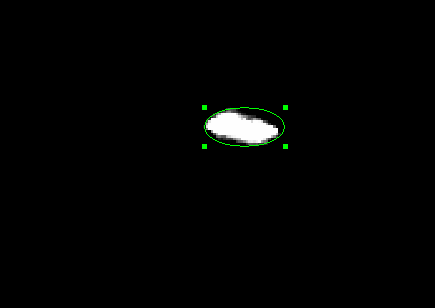
\includegraphics[width=0.45\textwidth]{Images/Ellipse_region.png}
    \caption{Description of the figure.}
    \label{fig:example}
\end{figure}

\section{Conclusions}
Discuss the main findings and potential future extensions of the work.

\section*{Acknowledgments}
Optional: mention people or institutions that supported the project.

\bibliography{ref}  % references.bib file

\end{document}
